% TeX compilation engine: pdfLaTeX
\documentclass[aspectratio=169]{beamer}

\usetheme{Frankfurt}
\usepackage[T2A]{fontenc}
\usepackage[utf8]{inputenc}
\usepackage[russian,english]{babel}
\usepackage{graphicx}

\title{Новая концепция интеграла,\\предложенная Лебегом, и ее развитие}
\author{Власов Максим Сергеевич, студент группы 3823М1ПМкн}
\institute[ННГУ]{Нижегородский государственный университет им. Н.И. Лобачевского}
\date{04.12.2024}

\begin{document}

\begin{frame}
\maketitle
\end{frame}

\begin{frame}
\frametitle{Содержание}
\tableofcontents
\end{frame}

\section*{Введение}

\begin{frame}
\frametitle{Введение}
Необходимость интегрального исчисления:
\begin{itemize}
    \item нахождение площади под кривой
    \item нахождение пройденного пути при неравномерном движении
    \item нахождение массы неоднородного тела
    \item восстановление функции по её производной
\end{itemize}
\end{frame}

\begin{frame}
\frametitle{Введение}
\begin{columns}[c]
    \begin{column}{0.45\textwidth}
        Подходы к интегрированию:
        \begin{itemize}
            \item Интеграл Римана
            \item Интеграл Лебега
        \end{itemize}
    \end{column}
    \begin{column}{0.45\textwidth}
        \includegraphics[width=0.8\textwidth]{images/integral_intro.png}
    \end{column}
\end{columns}
\end{frame}

\section{Интеграл Римана}

\begin{frame}
\frametitle{Интеграл Римана}
\begin{columns}[c]
    \begin{column}{0.45\textwidth}
        Площадь криволинейной трапеции, ограниченной графиками:

        $$
        y = 0, y = f(x), x = a, x = b
        $$

        Формализация понятия площади под графиком некоторой функции $f(x)$:

        $$
        \sigma = \sum_i f(\xi_i) \Delta x_i
        $$
    \end{column}
    \begin{column}{0.45\textwidth}
        \includegraphics[width=\textwidth]{images/riemann_integral.png}
    \end{column}
\end{columns}
\end{frame}

\begin{frame}
\frametitle{Определение интеграла Римана}
\begin{columns}[c]
    \begin{column}{0.45\textwidth}
        \begin{itemize}
            \item функция $f(x)$ определена на области $[a; b]$ почти всюду
            \item область разбита на $n$ интервалов шириной $\Delta x_i$, в каждом из которых выбрана точка $\xi_i$
            \item $n \rightarrow \infty$, $\Delta x \rightarrow 0$
        \end{itemize}

        $$
        \int\limits_a^b f(x) dx = \lim_{n \rightarrow \infty} \sum_{i = 1}^n f(\xi_i) \Delta x_i
        $$
    \end{column}
    \begin{column}{0.45\textwidth}
        \includegraphics[width=\textwidth]{images/riemann_integral.png}
    \end{column}
\end{columns}
\end{frame}

\begin{frame}
\frametitle{Особенности интеграла Римана}
\begin{itemize}
    \item применим к функциям, которые определены на конечном отрезке и ограничены на нем (точки разрыва, если есть, должны образовывать конечное или счетное множество нулевой меры)
    \item не определен для функций, разрывных на бесконечном множестве точек, даже если эти точки образуют множество с нулевой мерой
    \item не подходит для задач, требующих переход к пределу последовательности функций
\end{itemize}
\end{frame}

\section{Интеграл Лебега}

\begin{frame}
\frametitle{Интеграл Лебега}
\begin{columns}[c]
    \begin{column}{0.55\textwidth}
        \begin{itemize}
            \item Возможность работы с функциями, определенными на произвольных множествах
            \item Разбиение области значений функции $f(x)$, а не области определения $[a; b]$
            \item Использование меры Лебега $\mu$ для множеств (длина, площадь, объем)
        \end{itemize}
    \end{column}
    \begin{column}{0.35\textwidth}
        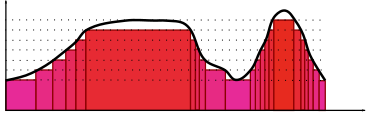
\includegraphics[width=\textwidth]{images/lebesgue_integral.jpg}
    \end{column}
\end{columns}
\end{frame}

\begin{frame}
\frametitle{Определение интеграла Лебега}
\begin{columns}[c]
    \begin{column}{0.55\textwidth}
        Разбиение области значений функции $f$ на меры Лебега $\mu$ вдоль горизонтальной оси:

        $$
        f^*(t) = \mu(\{x : f(x) > t\})
        $$

        Интеграл Лебега через интеграл Римана:

        $$
        \int\limits_a^b f(x) d\mu = \int\limits_0^\infty f^*(t)\,dt
        $$
    \end{column}
    \begin{column}{0.35\textwidth}
        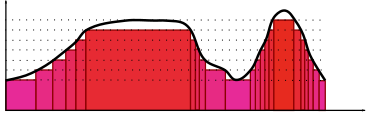
\includegraphics[width=\textwidth]{images/lebesgue_integral.jpg}
    \end{column}
\end{columns}
\end{frame}

\begin{frame}
\frametitle{Особенности интеграла Лебега}
\begin{itemize}
    \item Более широкий класс интегрируемых функций
    \item Удобство для работы с пределами функций
    \item Обработка разрывных функций
    \item Интегрирование по произвольным множествам
    \item Гибкость при преобразованиях функций
\end{itemize}
\end{frame}

\section{Приложения интеграла Лебега}

\begin{frame}
\frametitle{Приложения интеграла Лебега}
\begin{columns}[c]
    \begin{column}{0.5\textwidth}
        \begin{itemize}
            \item \textbf{Функциональный анализ:} исследование пространств Лебега $L^p$
            $$
            L^p(X, \mu) = \left\{ f: X \to \mathbb{R} \mid \int_X |f|^p \, d\mu < \infty \right\}
            $$
            \item \textbf{Вероятность и статистика:} сложные распределения случайных величин
            $$
            \mathbb{E}[X] = \int_\Omega X \, d\mathbb{P}
            $$
            ($\mathbb{P}$ -- мера вероятности)
        \end{itemize}
    \end{column}
    \begin{column}{0.5\textwidth}
        \begin{itemize}
            \item \textbf{Теория дифференциальных уравнений:} поиск слабых решений
            $$
            \int \phi(x) f'(x) \, dx = -\int \phi'(x) f(x) \, dx
            $$
            \item \textbf{Гармонический анализ:} преобразования с пределами
            $$
            \lim_{n \to \infty} \int f_n \, d\mu = \int \lim_{n \to \infty} f_n \, d\mu
            $$
            \item \textbf{Физика:} квантовая механика и статистическая механика
        \end{itemize}
    \end{column}
\end{columns}
\end{frame}

\section{Интеграл Лебега-Стилтьеса}

\begin{frame}
\frametitle{Интеграл Лебега-Стилтьеса}
\begin{columns}[c]
    \begin{column}{0.45\textwidth}
        Обобщение интегралов Лебега и Римана, которое позволяет интегрировать измеримую функцию $f(x)$ относительно произвольной монотонной функции $g(x)$ в качестве меры:

        $$
        \int\limits_a^b f(x) \, dg(x)
        $$
    \end{column}
    \begin{column}{0.45\textwidth}
        \includegraphics[width=\textwidth]{images/stieltjes_integral.png}
    \end{column}
\end{columns}
\end{frame}

\section*{Заключение}

\begin{frame}
\frametitle{Заключение}
\begin{itemize}
    \item \textbf{Интеграл Римана} -- эффективный инструмент для непрерывных и ограниченных функций.
    \item \textbf{Интеграл Лебега} можно применять для более широкого класс функций, например, определенных на множествах со сложной структурой или с разрывами на бесконечном множестве.
    \item Интеграл Лебега позволяет решать сложные задачи в различных разделах математического анализа, физики, теории вероятностей.
    \item Обобщения этих подходов, например, \textbf{интеграл Лебега-Стилтьеса}, открыли новые горизонты для исследований в математике и смежных областях.
\end{itemize}
\end{frame}

\end{document}
